%This is a Latex file.
\documentclass[12pt]{article}

\usepackage{amsmath, amssymb, amsthm, amscd, amsfonts, dsfont}
\usepackage{mathrsfs}
\usepackage{graphicx}
\usepackage{verbatim}
\usepackage{enumerate}
\usepackage{url,hyperref}
\usepackage{comment}
\usepackage{multicol}
\usepackage{latexsym,fancyhdr}
\usepackage[margin=1in]{geometry}
\usepackage{lastpage} % Required to determine the last page for the footer
\usepackage{tikz}
\usepackage{charter}
\usepackage{bbold}

\parindent 0pt

\pagestyle{fancy} \lhead{\sf MTH 415} \chead{\sf Homework \#3}
\rhead{\sf Due: Tuesday 03/31/2020} \lfoot{} \cfoot{} \rfoot{}

\newcommand{\C}{\mathbb{C}}
\newcommand{\R}{\mathbb{R}}
\newcommand{\Q}{\mathbb{Q}}
\newcommand{\Z}{\mathbb{Z}}
\newcommand{\N}{\mathbb{N}}

\renewcommand{\AA}{\mathcal{A}}
\newcommand{\BB}{\mathcal{B}}
\newcommand{\CC}{\mathcal{C}}
\newcommand{\DD}{\mathcal{D}}
\newcommand{\RR}{\mathcal{R}}
\renewcommand{\SS}{\mathcal{S}}
\newcommand{\TT}{\mathcal{T}}

\newcommand{\wts}[1]{\textit{\textcolor{blue}{WTS: #1}}\\}
\newcommand{\pg}{\textit{\textcolor{green}{PG: }}}
\newcommand{\pn}{\textit{\textcolor{yellow}{PN: }}}
\newcommand{\pb}{\textit{\textcolor{orange}{PB: }}}

\begin{document}
	\begin{enumerate}
		
		\item[2.23] Let $\mathcal{T}$ be the collection of subsets of $\mathbb{R}$ consisting of the empty set and every set whose complement is countable.\\
		\\
		(a) Show that $\mathcal{T}$ is a topology on $\R$. ( It is called the countable complement topology.)\\
		\\
		(i) \wts{$ \varnothing\in \TT, R\in\TT $}
		By definition, $ \varnothing\in\TT $ and $ R^\complement=\R-\R=\varnothing $.Hence, $ \R\in\TT $ and $ \varnothing\in\TT $\\\\
		(ii)\wts{The finite intersection of open sets is an open set}
		Let $ \{U_n\}_{n\in \Z^+} $ be an finite collection of non-empty open sets in $ \TT $. \\
		Notice, $ \R -\bigcap^n_{i=1} U_i = \bigcup^n_{i=1} \R - U_i  $. Since each $\R-U_i$ is countable, $ \bigcup^n_{i=1} \R - U_i   $ must be countable.\\
		Thus,  $\R -\bigcap^n_{i=1} U_i$ is countable.\\
		Therefore, The finite intersection of open sets is an open set.\\
		\\(iii)\wts{The union of arbitrary open sets is an open set}
		Let $ \{U_i\}_{i\in I} $ be an arbitrary collection of non-empty open sets in $ \TT $. \\
		Notice, $ \R -\bigcup_{i\in I} U_i = \bigcap_{i\in I} \R - U_i  $. Since the intersection of countable sets is countable, we have that $ \bigcap_{i\in I} \R- U_i $ is countable. \\
		Thus, $ \R-\bigcup_{i\in I} U_i  $ is countable.\\
		Therefore, the union of arbitrary open sets is an open set.\\
		\\
		Therefore, $ \TT $ is a topology on $ \R $.
		\\(b) Show that the point 0 is a limit point of the set $A=\mathbb{R}-\{0\}$ in the countable complement topology.\\
		\wts{if $\forall U\in\TT$ such that $0\in U$, $U\cap (A-0) \not= \varnothing$, then $0$ is a limit point of $A$.}
		Let $ U\in\TT $ such that $ 0\in U $ and define $ A:= \R-\{0\} $. Note, $ A $ is countable and so $ A\in \TT $. Recall, the set of irrational numbers. In $ \R $, the set of irrational numbers is uncountable and cannot be a complement of $ A $ or $ U $. So, $ A $ and $ U $ contain uncountably many irrational numbers. Hence, $ \exists i\in\mathbb{I} $ such that $ i\in U\cap A $.\\
		Thus, $ 0 $ is a limit point of $ A $.\\
		Therefore, the point 0 is a limit point of the set $A=\mathbb{R}-\{0\}$ in the countable complement topology.\\
		
		(c) Show that in $A=\R-\{0\}$ there is no sequence converging to 0 in the countable complement topology.\\
		Let $ (x_n) $ be a sequence in $ \R-\{0\} $ and define $ U:=\R-\{x_n|n\in\Z^+\} $. Note, $ (x_n) $ is countable and so $ U\in\TT $. We also know that $ 0\in U $ and $ U $ does not have any elements from $ (x_n) $ from our definition of the sequence $ \R-\{0\} $. \\
		Thus, $ (x_n) $ does not converge to $ 0 $.\\
		Therefore, in $A=\R-\{0\}$ there is no sequence converging to 0 in the countable complement topology.
		\item[2.26] Determine the boundary of each of the following subsets of $\mathbb{R}^{2}$ in the standard topology:\\
		(a) $\quad A=\left\{(x, 0) \in \mathbb{R}^{2} | x \in \mathbb{R}\right\}$\\
		\begin{align*}
			\partial A &= Cl(A)-Int(A)\\
			X\text{-Axis}&= X\text{-Axis}-\varnothing
		\end{align*}
		(b) $\quad B=\left\{(x, y) \in \mathbb{R}^{2} | x>0, y \neq 0\right\}$\\
		\begin{align*}
			\partial B &= Cl(B)-Int(B)\\
			\{(x,y)|x=0\}\cup\{(x,y)|x>0,y=0\}&=\{(x,y)|x\geq 0\}-B
		\end{align*}
		(c) $\quad C=\left\{\left(\frac{1}{n}, 0\right) \in \mathbb{R}^{2} | n \in \mathbb{Z}_{+}\right\}$\\
		\begin{align*}
			\partial C &= Cl(C)-Int(C)\\
			\{(x,0)|0<x\leq 1\}&=\{(x,0)|0<x\leq 1\}-\varnothing
		\end{align*}
		(d) $D=\left\{(x, y) \in \mathbb{R}^{2} | 0 \leq x^{2}-y^{2}<1\right\}$\\
		\begin{align*}
			\partial D &= Cl(D)-Int(D)\\
			D&=D-\varnothing
		\end{align*}
		\item[2.28] Prove Theorem 2.15 : Let $A$ be a subset of a topological space $X .$\\
		\\(a) $\partial A$ is closed.\\
			Observe,
			\begin{align*}
				 \partial A &= Cl(A)-Int(A)\\
				 \partial A &= Cl(A)\cap (X-Int(A))  
			\end{align*}
			Notice, the complement of $ Int(A) $ is closed and $Cl(A)$ is closed by definition. Thus, the intersection of closed sets is a closed set.\\
			Therefore, $ \partial A $ is closed.
		\\(b) $\partial A=Cl(A) \cap Cl(X-A)$\\
			Observe,
			\begin{align*}
				\partial A &= Cl(A)-Int(A)\\
						   &= Cl(A)\cap(X-Int(A))\\
						   &= Cl(A)\cap Cl(X-A) \text{ by theorem 2.6(ii)}
			\end{align*}
			Therefore,  $\partial A=Cl(A) \cap Cl(X-A)$\\
		\\(c) $\partial A \cap \operatorname{Int}(A)=\varnothing$\\
			Observe,
			\begin{align*}
				\partial A &= Cl(A)-Int(A)\\
				\partial A \cap Int(A) &= (Cl(A)-Int(A))\cap Int(A)\\
				\partial A \cap Int(A) &= \varnothing
			\end{align*}
			Therefore,  $\partial A \cap \operatorname{Int}(A)=\varnothing$\\
		\\(d) $\partial A \cup \operatorname{Int}(A)=C l(A)$\\
			Observe,
			\begin{align*}
				\partial A &= Cl(A)-Int(A)\\
				\partial A \cup Int(A) &= (Cl(A)-Int(A))\cup Int(A)\\
				\partial A \cup Int(A) &= Cl(A)
			\end{align*}
		Therefore, $\partial A \cup \operatorname{Int}(A)=C l(A)$\\
		\\(e) $\partial A \subset A$ if and only if $A$ is closed.\\
		Observe,
		\begin{align*}
			\partial A \subset A \Leftrightarrow Cl(A)-Int(A)\subset A \Leftrightarrow Cl(A)=A \Leftrightarrow A \text{ is closed}
		\end{align*}
		Therefore, $\partial A \subset A$ if and only if $A$ is closed.\\
		\\(f) $\partial A \cap A=\varnothing$ if and only if $A$ is open.\\
		Observe,
		\begin{align*}
			\partial A \cap A =\varnothing = \partial A \cap Int(A) \Leftrightarrow Int(A)=A \Leftrightarrow A \text{ is open}
		\end{align*}
		 Therefore, $\partial A \cap A=\varnothing$ if and only if $A$ is open.\\
		\\(g) $\partial A=\varnothing$ if and only if $A$ is both open and closed.\\
		Observe,
			\begin{align*}
				\partial A=\varnothing \Leftrightarrow Cl(A)-Int(A)= \varnothing \Leftrightarrow Cl(A)=Int(A) \Leftrightarrow A \text{ is open and closed}
			\end{align*}
		Therefore, $\partial A=\varnothing$ if and only if $A$ is both open and closed.\\
		\item[3.01] Let $X=\left\{(x, 0) \in \mathbb{R}^{2} | x \in \mathbb{R}\right\},$ the $x$ -axis in the plane. Describe the topology that $X$ inherits as a subspace of $\mathbb{R}^{2}$ with the standard topology.\\
		The topology is comprised of open intervals on the $x$-axis. The subspace is $ \R $ with the standard topology.
		
		\item[3.02] Let $Y=[-1,1]$ have the standard topology. Which of the following sets are open in $Y$ and which are open in $\mathbb{R} ?$
		$$
		\begin{array}{l}
		A=(-1,-1 / 2) \cup(1 / 2,1)  \text{ :: open in $ \R $; open in $ Y $}\\
		B=(-1,-1 / 2] \cup[1 / 2,1)  \text{ :: not open in $ \R $; not open in $ Y $} \\
		C=[-1,-1 / 2) \cup(1 / 2,1]  \text{ :: not open in $ \R $; open in $ Y $}\\
		D=[-1,-1 / 2] \cup[1 / 2,1]  \text{ :: not open in $ \R $; not open in $ Y $}\\
		E=\bigcup_{n=1}^{\infty}\left(\frac{1}{1+n}, \frac{1}{n}\right) \text{ :: open in $ \R $; open in $ Y $}
		\end{array}
		$$
		
		\item[3.03] Prove Theorem 3.4 : Let $X$ be a topological space, and let $Y \subset X$ have the subspace topology. Then $C \subset Y$ is closed in $Y$ if and only if $C=D \cap Y$ for some closed set $D$ in $X$.\\
		\begin{proof}
			Let $ X $ be topological space, $ Y\subset X $ have the subspace topology, and $ C\subset Y $ \\
		$(\Rightarrow)$ \wts{if $ C $ is closed in $ Y $ then $ C=D\cap Y $}
		Assume $ C $ is closed in $ Y $. Then $ Y-C $ is open in $ Y $. Since $ Y-C $ is open, there exists an open set $ U $ in $ X $, such that $ Y-C=Y\cap U $. As $ U $ is open, it follows that $ X-U $ is closed. Define $ D=X-U $ and hence $ D $ is closed in $ X $. Notice,
			\begin{align*}
				Y-C &= Y\cap U\\
				C &= Y- (Y\cap U)\\
				C &= Y-U\\
				C &= Y\cap(X-U)\\
				C &= Y\cap D\\
			\end{align*}
		Hence, $ C=D\cap Y $\\
		Thus, if $ C $ is closed in $ Y $, then $ C=D\cap Y $\\
		\\
		$(\Leftarrow)$ \wts{if $ D $ is a closed set in $ X $ and $ C=D\cap Y $, then $ C $ is closed in $ Y $}
		Assume $ D $ is a closed set in $ X $ and $ C=D\cap Y $. Since $ D $ is closed in $ X $, $ X-D $ is open in $ X $. Which means, by definition of a subspace topology, $ Y\cap(X-D) $ is open in $ Y $. Then, $ Y-(Y\cap(X-D)) $ is closed in $ Y $. Observe,
			\[Y-(\textcolor{purple}{Y\cap(X-D)})=(Y-\textcolor{purple}{Y})\cup (Y-\textcolor{purple}{(X-D)})=Y-\textcolor{purple}{(X-D)}=Y\cap D = C\]
		It follows that $ C $ is closed in $ Y $.\\
		\\
		Therefore, $C \subset Y$ is closed in $Y$ if and only if $C=D \cap Y$ for some closed set $D$ in $X$.
		\end{proof}
		
		\item[3.15] Prove Theorem 3.9: Let $X$ and $Y$ be topological spaces, and assume that
		$A \subset X$ and $B \subset Y .$ Then the topology on $A \times B$ as a subspace of the product
		$X \times Y$ is the same as the product topology on $A \times B,$ where $A$ has the subspace topology inherited from $X,$ and $B$ has the subspace topology inherited from $Y$.\\
		\begin{proof}
		  Let $X$ and $Y$ be topological spaces, and assume that $A \subset X$ and $B \subset Y .$ Using definition 3.6 and theorem 3.7, we have that $\BB_{X\times Y} = \{U\times V\ |U\in X, V\in Y \} $. Also, by definition of a subspace we have $ \BB_{A\times B}=\{(U\times V)\cap(A\times B) \} $. Observe,
		  \[(U\times V)\cap(A\times B)=(U\cap A)\times(V\cap B) \]
		  Note, $ U\cap A $ and $ V\cap B $ are bases elements for the subspace on $ A $ and $ B $ respectively. Then, $ \BB=\{(U\cap A)\times(V\cap B) \}$ is our basis for the product topology on $ A\times B $. Hence, by rewriting we see they are equivalent.\\
		  Therefore, the topology on $A \times B$ as a subspace of the product
		  $X \times Y$ is the same as the product topology on $A \times B,$ where $A$ has the subspace topology inherited from $X,$ and $B$ has the subspace topology inherited from $Y$.\\
 		\end{proof}
		
		\item[3.16] Let $S^{2}$ be the sphere, $D$ be the disk, $T$ be the torus, $S^{1}$ be the circle, and $I=[0,1]$ with the standard topology. Draw pictures of the product spaces $S^{2} \times I, T \times I, S^{1} \times I \times I,$ and $S^{1} \times D$\\
		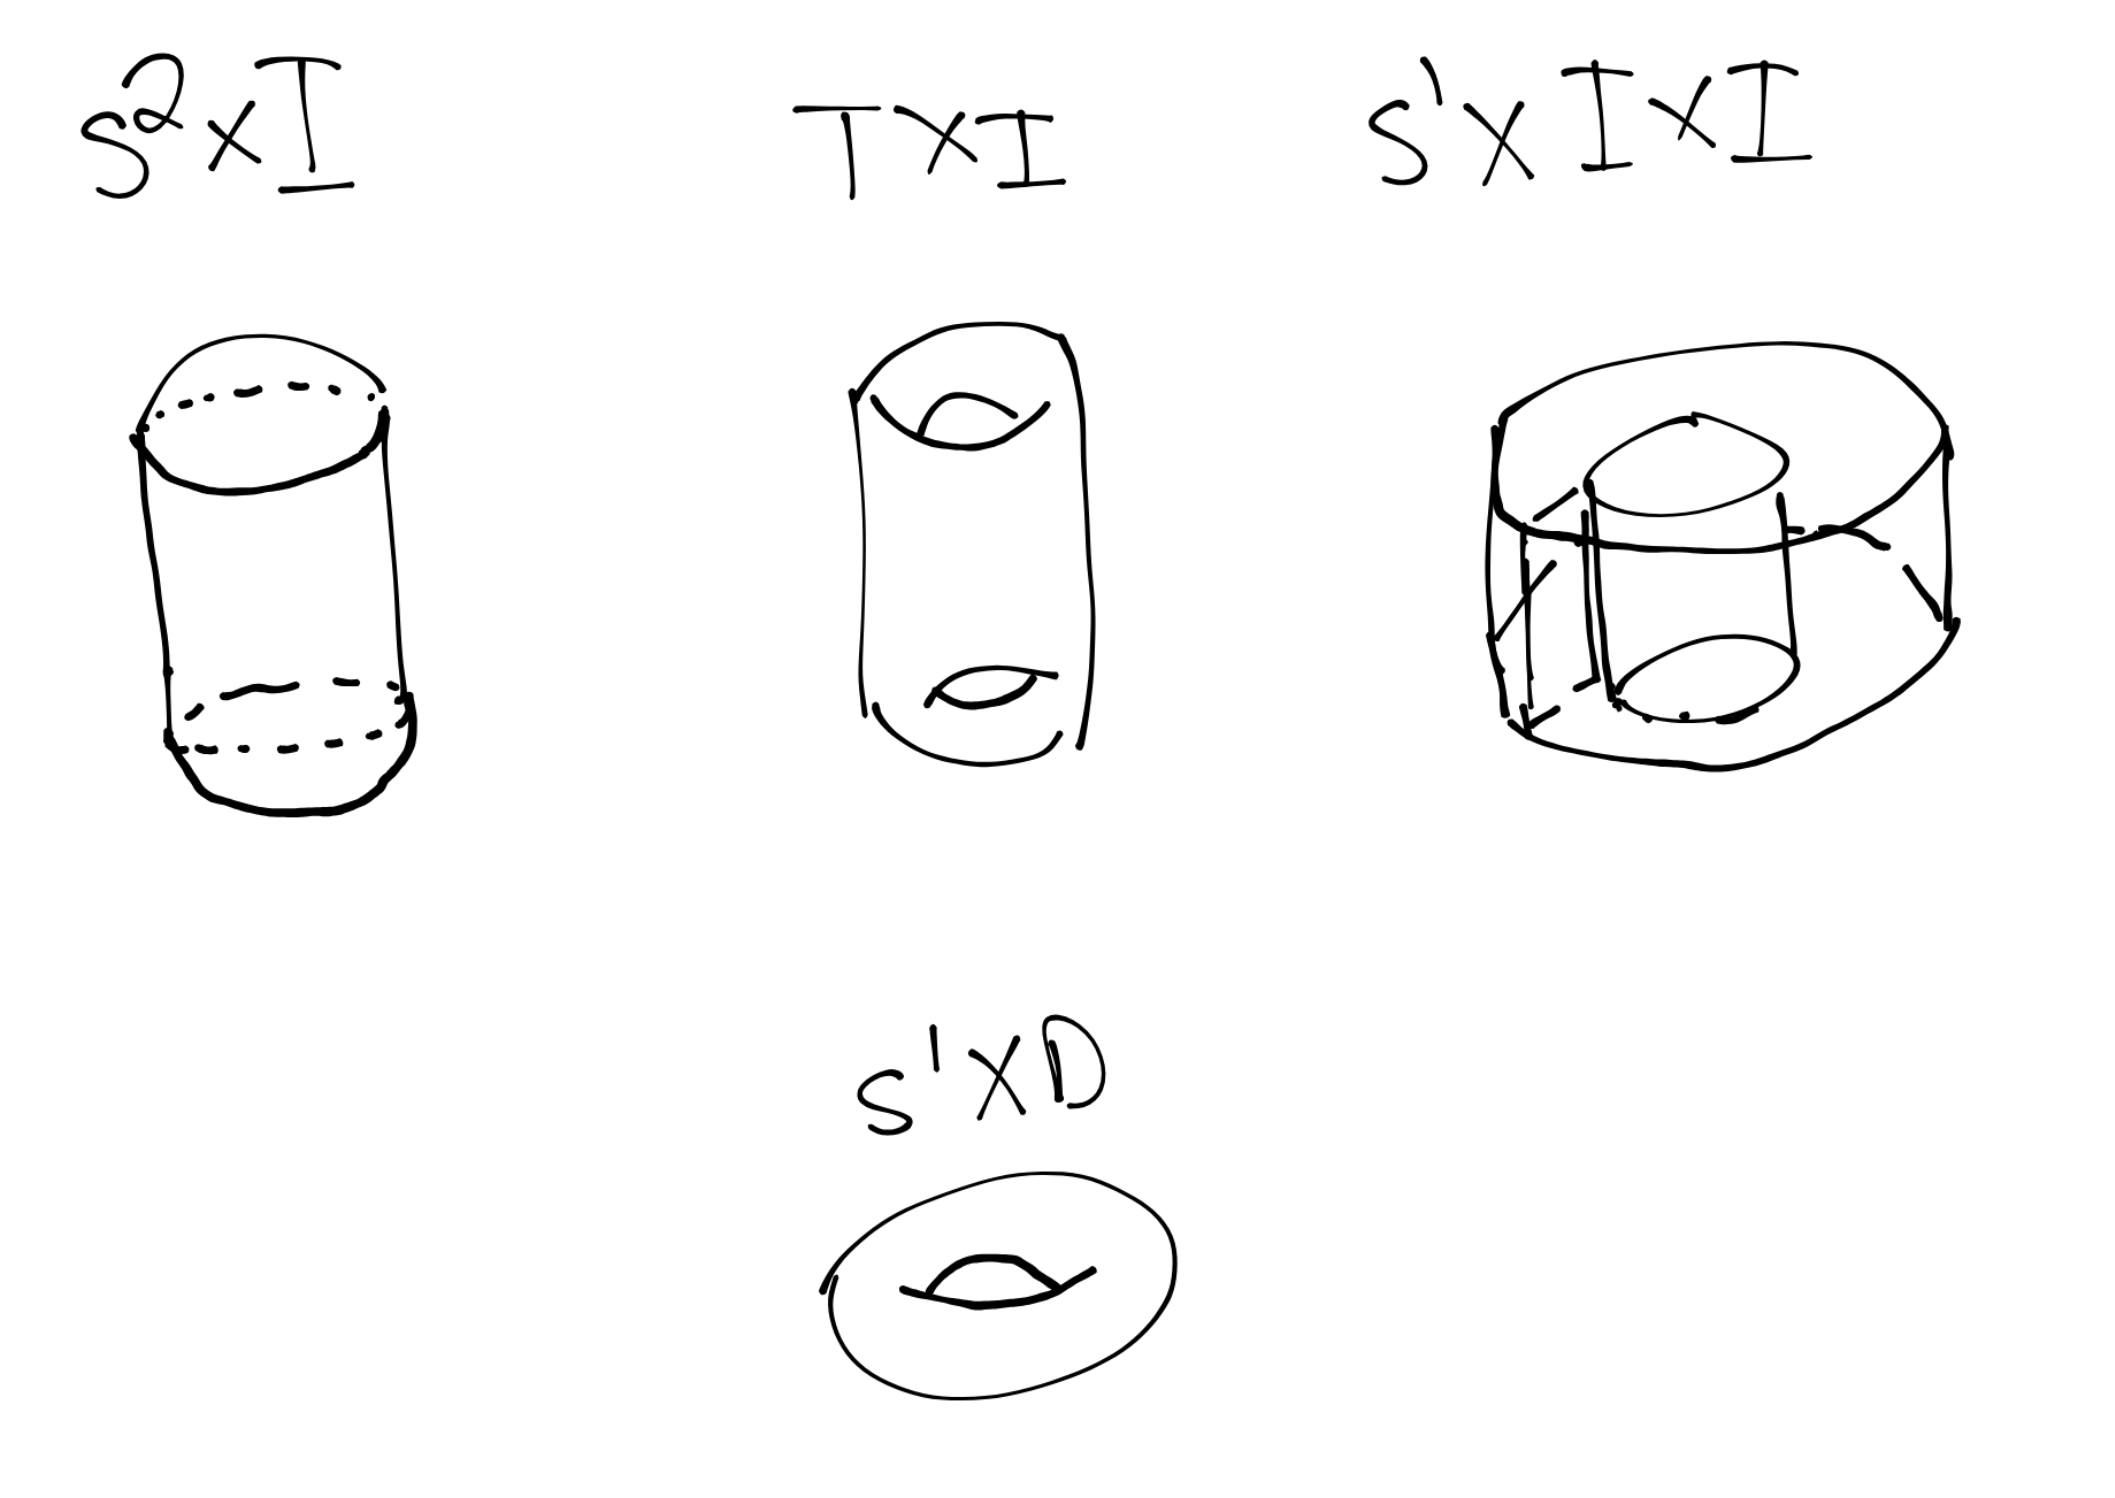
\includegraphics[scale=.12]{3.16.png}
		\item[3.18] Show that if $X$ and $Y$ are Hausdorff spaces, then so is the product space $X \times Y$.
		\begin{proof}
			Let $ X $ and $ Y $ be Hausdorff spaces and $ X\times Y $ be their product space.\\
			\wts{$ X\times Y $ is Hausdorff}
			\wts{$ \forall (x,y),(x',y') \in X\times Y $ such that $ x\not=x' $ or $ y\not=y' $, $ \exists U,V\in\TT_{X\times Y}$ such that $ (x,y)\in U $, $ (x',y')\in V $ and $ U\cap V=\varnothing $}
			Let $ (x,y),(x',y')\in X\times Y $ with $ x\not=x' $ or $ y\not=y'$. Without loss of generality, assume $ x\not=x' $. Since $ X $ is Hausdorff, $ \exists U,U'\in \TT_X $ such that $ x\in U $, $ x'\in U' $ and $ U\cap U' =\varnothing $. Notice, $ U\times Y, U'\times Y \in \TT_{X\times Y}$ and $ (x,y)\in U\times Y $, $ (x',y')\in U' $. Observe,
			\[(U\times Y)\cap(U'\times Y) = (U\cap U')\times Y = \varnothing \times Y = \varnothing  \]
			Thus, we have found two disjoint neighborhoods of two points in $ X\times Y $.\\
			Hence, by definition of Hausdorff, $ X\times Y $ is also Hausdorff.\\
			Therefore, if $X$ and $Y$ are Hausdorff spaces, then so is the product space $X \times Y$.
		\end{proof}
		
		\item[3.19] Show that if $A$ is closed in $X$ and $B$ is closed in $Y$, then $A \times B$ is closed in $X \times Y$.\\
		
		\begin{proof}
		Let $ A $ be a closed subset in $ X $ and $ B $ be a closed subset in $ Y $.\\
		\wts{$ A\times B $ is closed in $ X\times Y $}	
		\wts{$ X\times Y - A\times B$ is open}
		\wts{$((X-A)\times Y) \cup (X\times (Y - B))$ is open}	
		Then, $ X-A $ is open in $X$ and $ Y-B $ is open in $ Y $.\\
		Let $ (x,y)\in X\times Y - A\times B $. Then $ (x,y)\in X\times Y $ and $ (x,y)\not\in A\times B $. So, $ x \not\in A $ or $ y \not \in B $. Thus, $ x\in X-A $ or $ y\in Y-B $.Since $X-A$ is open in $X$, $ (X-A)\times Y $ is open in $ X\times Y $. Similarly, $ Y-B $ is open in $Y$, $ X\times(Y-B) $ must be open in $ X\times Y $.\\
		So, $ (x,y)\in ((X-A)\times Y)\cup (X\times(Y-B)) $
		Hence, $ X\times Y - A\times B $ is open\\
		Thus, $ A\times B $ is closed in $ X\times Y $\\
		Therefore, if $A$ is closed in $X$ and $B$ is closed in $Y$, then $A \times B$ is closed in $X \times Y$.\\
		\end{proof}
		
	\end{enumerate}
\end{document}